\documentclass{article}
\setlength{\parskip}{5pt} % esp. entre parrafos
\setlength{\parindent}{0pt} % esp. al inicio de un parrafo
\usepackage{listings} % listings
\usepackage{color} %colores
\usepackage{amsmath} % mates
\usepackage[sort&compress,numbers]{natbib} % referencias
\usepackage{url} % que las URLs se vean lindos
\usepackage[top=15mm,left=20mm,right=20mm,bottom=25mm]{geometry} % margenes
\usepackage{hyperref} % ligas de URLs
\usepackage{graphicx} % poner figuras
\usepackage[spanish]{babel} % otros idiomas

\author{Claudia Lizeth Hern\'andez Ram\'irez} % author
\title{Homework 8 - Sistema de Urnas} % titulo
\date{\today}

\definecolor{mypurple}{rgb}{0.305, 0.066, 0.592}
\definecolor{mygray}{rgb}{0.976, 0.980, 0.980}
\definecolor{myorange}{rgb}{0.933, 0.305, 0.090}
\lstset{ 
  backgroundcolor=\color{mygray},
  commentstyle=\color{myorange},
  keywordstyle=\color{mypurple}, 
  numberstyle=\tiny\color{myorange}
  stringstyle=\color{mypurple}, 
  breaklines=true,
}


\begin{document} % inicia contenido

\maketitle % cabecera

% RESUMEEEEEEEEEEEEEEEN
\begin{abstract} % resumen
  \centering
Conforme se aumentan las iteraciones, el porcentaje de filtraci\'on disminuye considerablemente. El mejor porcentaje de filtraci\'on resulta en la primer iteraci\'on.
  
\end{abstract}


% INTRODUCCIOOOOOOOOOOOON
\section{Introducci\'{o}n}\label{intro} % seccion y etiqueta
Simulando un sistema de filtraci\'on de aguas residuales, se formas c\'umulos de part\'iculas las cuales pueden fragmentarse o unirse entre ellas. Se determina un n\'umero fijo de part\'iculas \texttt{n}, en este caso \texttt{100000} y se estar\'an variando los c\'umulos \texttt{k} entre \texttt{100}, \texttt{200} y \texttt{400}, el tamaño del \texttt{filtro} ser\'a igual a \texttt{c}, es decir que tamaño \texttt{cr\'itico}.



% DESARROLLOOOOOOOOOOOO
\section{Desarrollo}\label{desarrollo} % Desarrollo de la tarea

Se trabajo con el c\'odigo base que se explic\'o en clase \cite{Cbase}. En un inicio se agregaron dos ciclos \texttt{FOR}, el primero para variar los c\'umulos, denomiados en el c\'odigo como \texttt{grupo}; el segundo ciclo \texttt{FOR} es referente a las r\'eplicas que realizar\'a el programa, en esta ocasi\'on fueron \texttt{50} r\'eplicas.


\begin{lstlisting}[language=R, caption= Segmento de c\'odigo ciclos \texttt{FOR} para c\'umulos y repeticiones.]

grupo <- c(100, 200, 400)
replica = 1:50
n <- 100000
datos = data.frame()

for (k in grupo){
  for (reply in replica){
    originales <- rnorm(k)
    cumulos <- originales - min(originales) + 1
    cumulos <- round(n * cumulos / sum(cumulos))

\end{lstlisting}

Posteriormente, bas\'andome en los ejemplos vistos en clase \cite{fragmento}, se gener\'o un c\'odigo para sacar el porcentaje de filtraci\'on exitoso.

.
\begin{lstlisting}[language=R, caption= Segmento de c\'odigo para filtrado exitoso.]
filtrados = freq[freq$tam >= c,]
      filtrados$cont = filtrados$tam * filtrados$num
      f = sum(filtrados$cont) # particulas removidas
      porcentaje = (f/n) * 100 # porcentaje exitosamente filtrado
      resultado = c(k, reply, paso, porcentaje)
      datos = rbind(datos, resultado)
      names(datos) = c("k", "Replica", "Iteracion", "Filtrado")
\end{lstlisting}

Todo esto dentro de los ciclos \texttt{FOR} que se generaron en un inicio.


Despu\'es apliqu\'e pruebas de normalidad a mi datos.

\begin{lstlisting}[language=R, caption= Segmento de c\'odigo para prueba de normalidad Shapiro-Wilk.]

#Estadistica prueba de normalidad - 
      #con p menor a 0.05 se rechaza hipotesis nula H0
      #H0: las medias son iguales en todos los grupos.
      #H1: existen diferencias significativas entre las medias de los grupos.
tapply(datos$Filtrado, datos$k, shapiro.test)
\end{lstlisting}

De esta prueba se obtuvieron los datos expresados en el cuadro \ref{cuadro 1} (En la literatura podemos encontrar que diversos autores establecen que en pruebas de normalidad para aceptar la hip\'otesis nula el valor de \texttt{P} debe ser mayor al 0.05, es decir mayor al 5\%).

\begin{table}[ht]
    \centering
    \caption{Resultados obtenidos de prueba de normalidad de Shapiro.} 
    \begin{tabular}{|c|c|c|c|}
    \hline
    C\'umulo & W value & P value & ¿Se acepta H0?  \\
    \hline
    100 & 0.41416 & $2.2\times 10^{-16}$ & no \\
    \hline 
     200 & 0.83836 & $2.2\times 10^{-16}$ & no  \\
    \hline 
    400 & 0.99943 & 0.6802 & s\'i \\
    \hline 
\end{tabular}
    \label{cuadro 1}
\end{table}

Con la informaci\'on obtenida en las pruebas de normalidad, podemos seguir con la prueba estad\'istica. En esta ocasi\'on recurriremos a la prueba de \texttt{Kruskal-Wallis} \cite{Kruskal}.

\begin{lstlisting}[language=R, caption= Segmento de c\'odigo para prueba de Kruskal-Wallis]
#PRUEBA ESTADISTICA
datos%>%
 group_by(k) %>%
  summarise(
    cantidad_de_participantes = n(),
    promedio = mean(Filtrado, na.rm = TRUE),
    desviacion_estandar = sd(Filtrado, na.rm = TRUE),
    varianza = sd(Filtrado, na.rm = TRUE)^2,
    mediana = median(Filtrado, na.rm = TRUE),
    rango_intercuartil =  IQR(Filtrado, na.rm = TRUE)
    )

kruskal.test(Filtrado ~ k, data = datos)
pairwise.wilcox.test(datos$Filtrado, datos$k)
\end{lstlisting}


De donde se obtuvieron los resultados expresados en el cuadro \ref{cuadro 2}, \ref{cuadro 3} y \ref{cuadro 4}.

\begin{table}[ht]
    \centering
    \caption{Resultados obtenidos de prueba Kruskal-Wallis.} 
    \begin{tabular}{|c|c|c|}
    \hline
    Chi cuadrada & DF & P  \\
    \hline
    6600.4 & 2 & $2.2\times 10^{-16}$ \\
    \hline
\end{tabular}
    \label{cuadro 2}
\end{table}

\begin{table}[ht]
    \centering
    \caption{Diferencias entre grupos. Kruskal-Wallis.} 
    \begin{tabular}{|c|c|c|c|c|c|c|c|c|c|}
    \hline
    "" & 100 & 200 \\
    \hline
    200 & $2\times 10^{-16}$ & "" \\
    \hline
    400 & $2\times 10^{-16}$ & $2\times 10^{-16}$ \\
    \hline
\end{tabular}
    \label{cuadro 3}
\end{table}


\begin{table}[ht]
    \centering
    \caption{Informaci\'on individual de los datos.} 
    \begin{tabular}{|c|c|c|c|c|c|c|}
    \hline
    Probabilidad & Qty. Participantes & promedio & Desv. Std. & Varianza & Mediana & Rango Intercuartil  \\
    \hline
    100 & 2500 & 2.26 & 6.20 & 38.4 & 0 & 1.01 \\
    \hline
    200 & 2500 & 27.6 & 3.36 & 11.3 & 27.0 & 3.07 \\
    \hline
    400 & 2500 & 49.9 & 1.38 & 1.90 & 49.9 & 1.86 \\
    \hline
\end{tabular}
    \label{cuadro 4}
\end{table}
\newpage

La informaci\'on presentada anteriormente puede visualizarse m\'as facilmente en las gr\'aficas \ref{Figura 1}, \ref{Figura 2} y \ref{Figura 3}.

\begin{figure}[ht] % figura
    \centering
    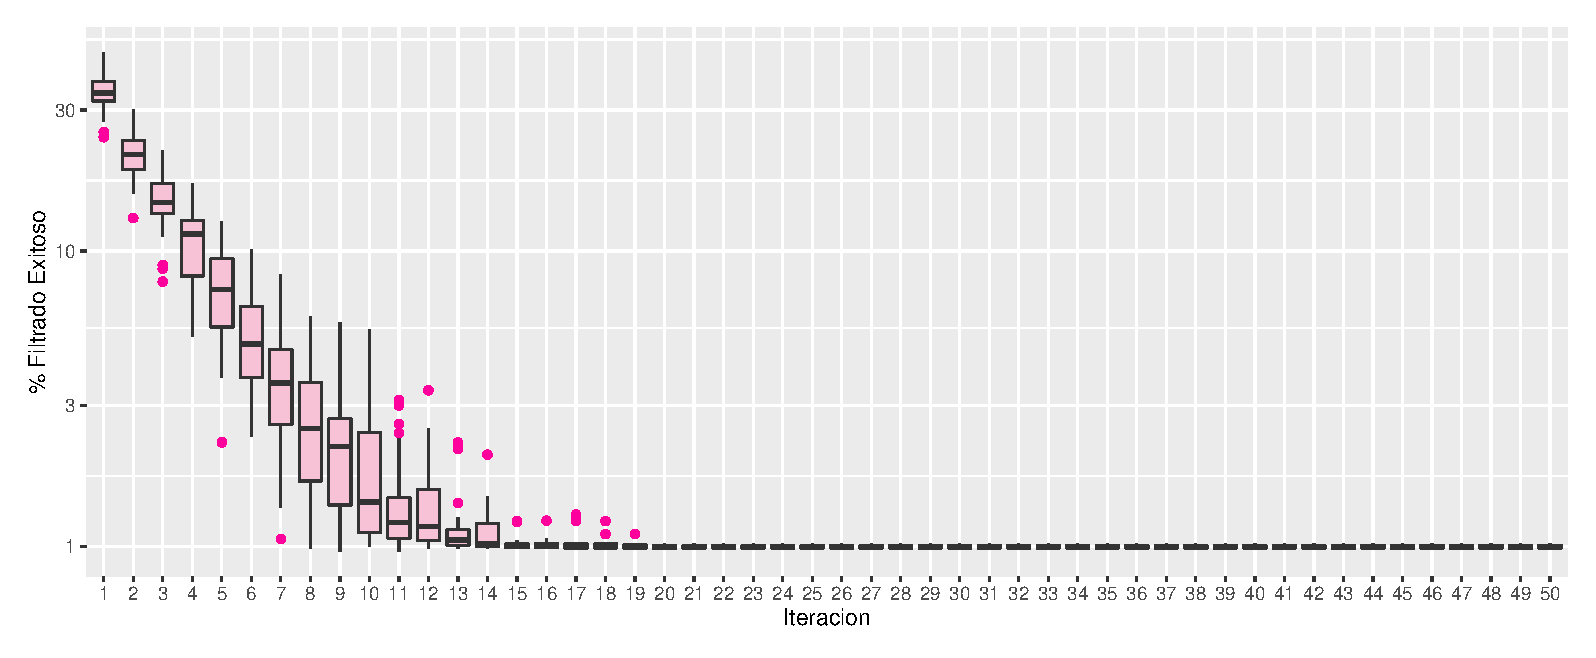
\includegraphics[width=150mm]{k100.eps} % archivo
    \caption{k = 100.}
    \label{Figura 1}
\end{figure}
\begin{figure}[ht] % figura
    \centering
    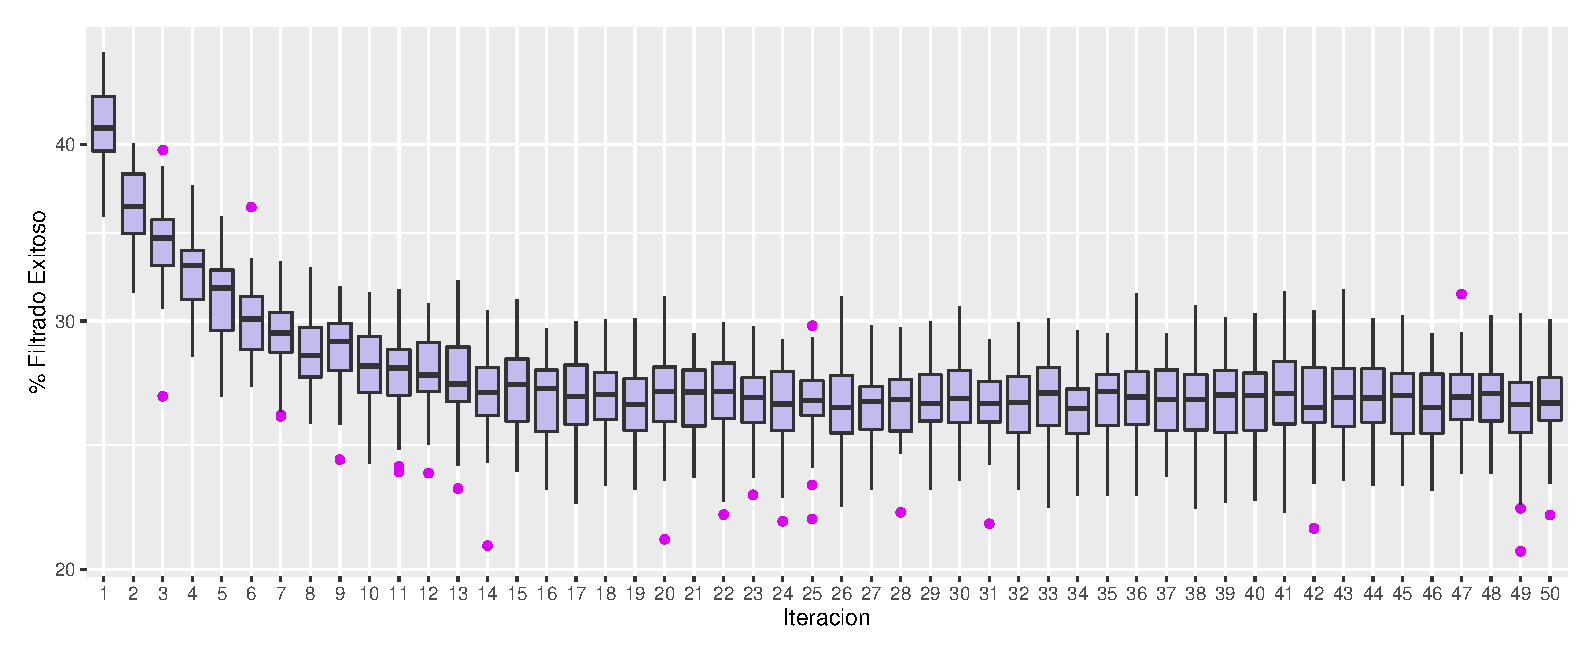
\includegraphics[width=150mm]{k200.eps} % archivo
    \caption{k = 200.}
    \label{Figura 2}
\end{figure}
\begin{figure}[ht] % figura
    \centering
    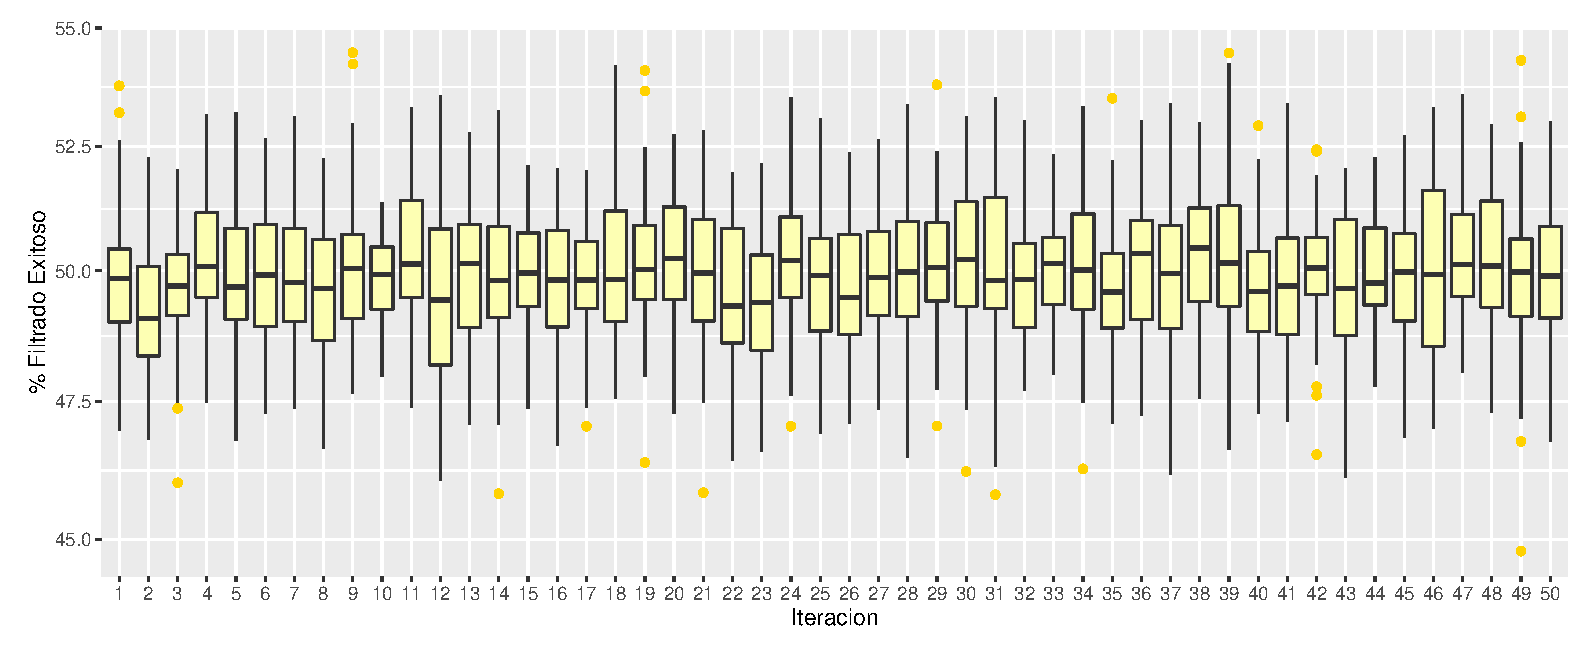
\includegraphics[width=150mm]{k400.eps} % archivo
    \caption{k = 400.}
    \label{Figura 3}
\end{figure}


\newpage

Considerando que 

-Hip\'otesis nula: hay diferencias en el porcentaje de filtraci\'on exitoso y las iteraciones.

-Hip\'otesis alternativa: no hay diferencias en el porcentaje de filtraci\'on exitoso y las iteraciones.

-Con un nivel de significancia igual a 0.05

Contamos con evidencia estad\'istica suficiente para rechazar la \texttt{hip\'otesis nula}.

%CONCLUSIOOOON
\section{Conclusi\'on}
Con base en las im\'agenes anteriores, podemos deducir que el porcentaje de filtraci\'on ir\'a disminuyendo conforme las iteraciones aumentan, sin embargo ocurre algo excepcional en el grupo de c\'umulos \texttt{k=400} ya que no se observa la misma tendencia que en los primeros dos grupos, \texttt{k=100} y \texttt{k=200}.
Ignorando dicho grupo, pareciera que el mejor resultado de filtraci\'on resulta de la primera iteraci\'on.



\bigskip 


\section{Reto 2 - Variar tamaño cr\'itico para validar cantidad de part\'iculas que quedan atrapadas en el filtro.}

Se modific\'o el tamaño de \texttt{c} que como se mencion\'o con anterioridad representa el tamaño cr\'itico. En esta ocasi\'on no tomar\'a el valor de la media sino, el valor del cuartil.

Aplicando el mismo c\'odigo que, en la tarea base, se obtienen las im\'agenes \ref{Figura 4}, \ref{Figura 5} y \ref{Figura 6}.

\begin{lstlisting}[language=R, caption= Segmento de c\'odigo para modificar valor del tamaño cr\'itico.]

assert(length(cumulos[cumulos == 0]) == 0) # que no haya vacios
    assert(sum(cumulos) == n)
    c <- median(cumulos)/2 # tamanio critico de cumulos
    d <- sd(cumulos) / 4 # factor arbitrario para suavizar la curva
    rotura <- function(x) {
      return (1 / (1 + exp((c - x) / d)))
    }
\end{lstlisting}
\newpage
\begin{figure}[ht] % figura
    \centering
    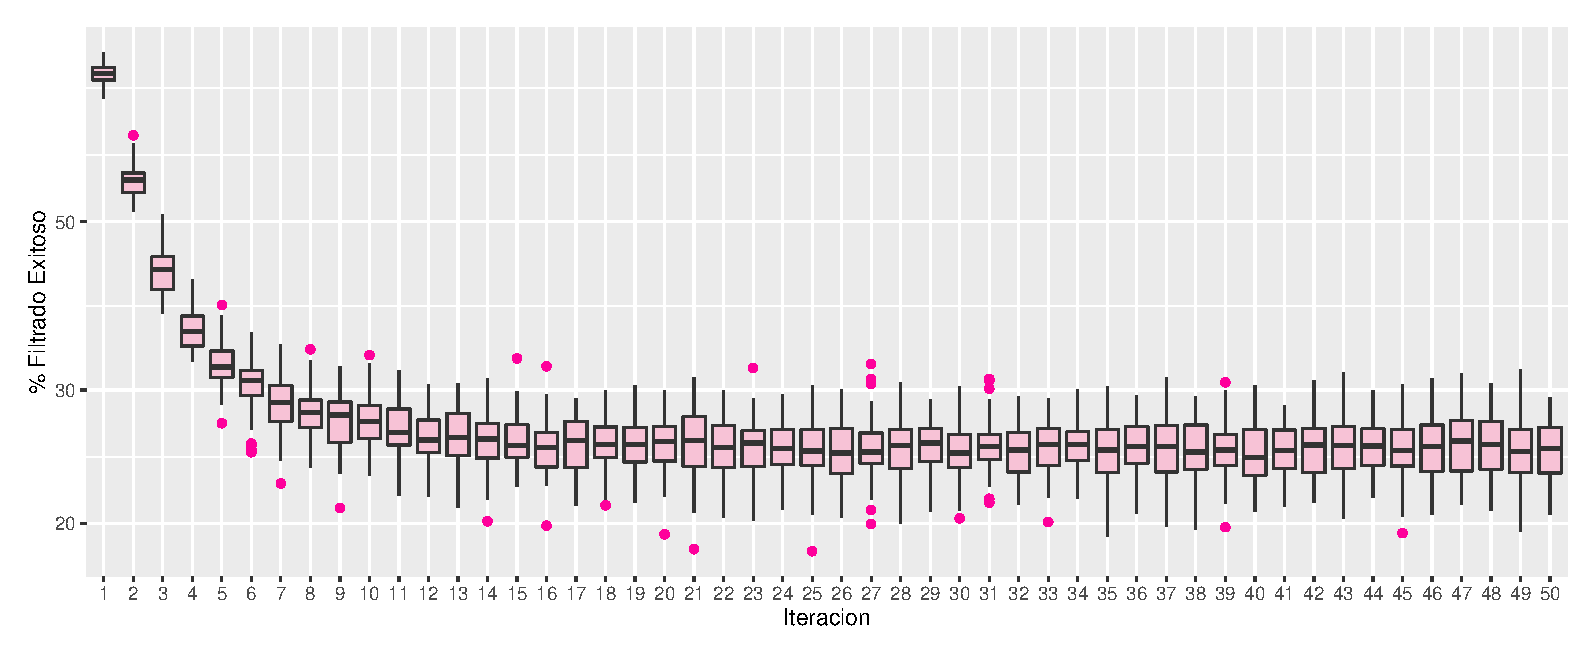
\includegraphics[width=150mm]{k100r2.eps} % archivo
    \caption{k = 100 R2.}
    \label{Figura 4}
\end{figure}

\begin{figure}[ht] % figura
    \centering
    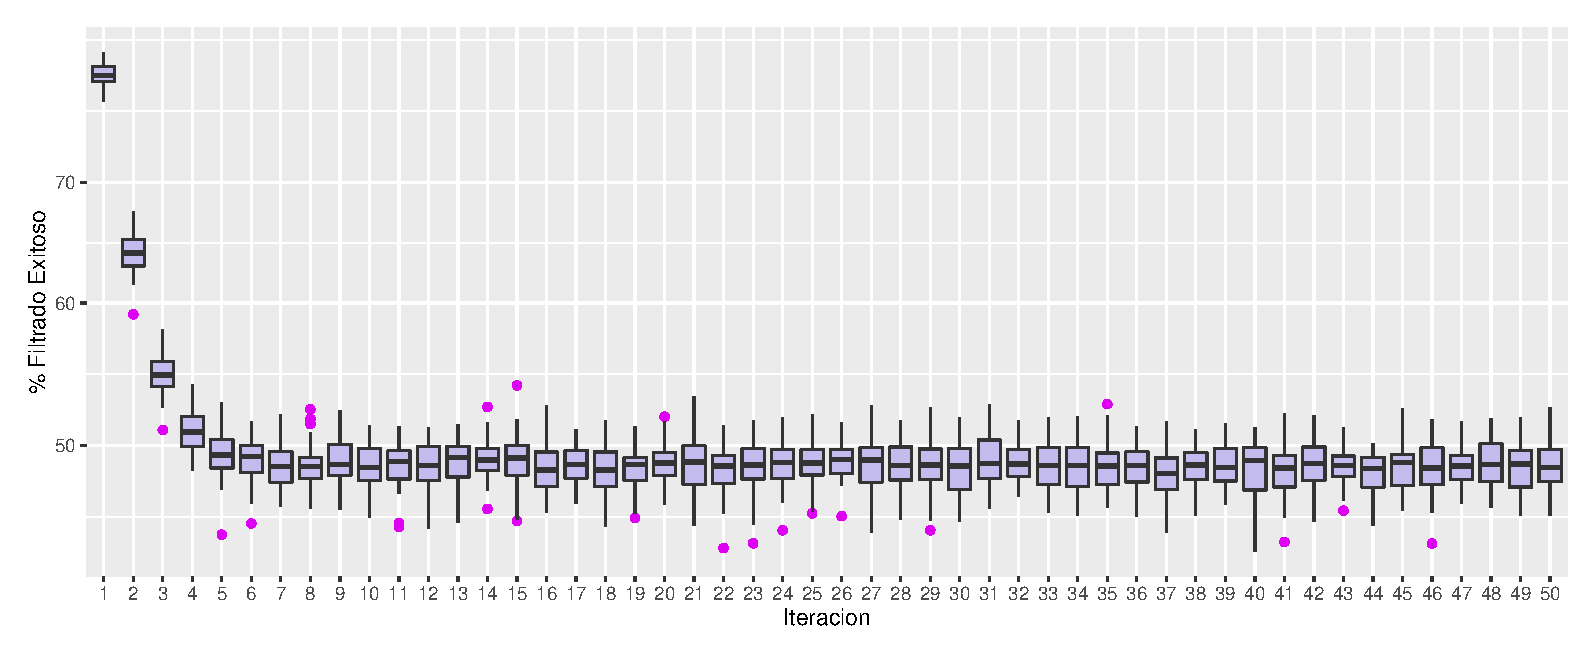
\includegraphics[width=150mm]{k200r2.eps} % archivo
    \caption{k = 200 R2.}
    \label{Figura 5}
\end{figure}

\begin{figure}[ht] % figura
    \centering
    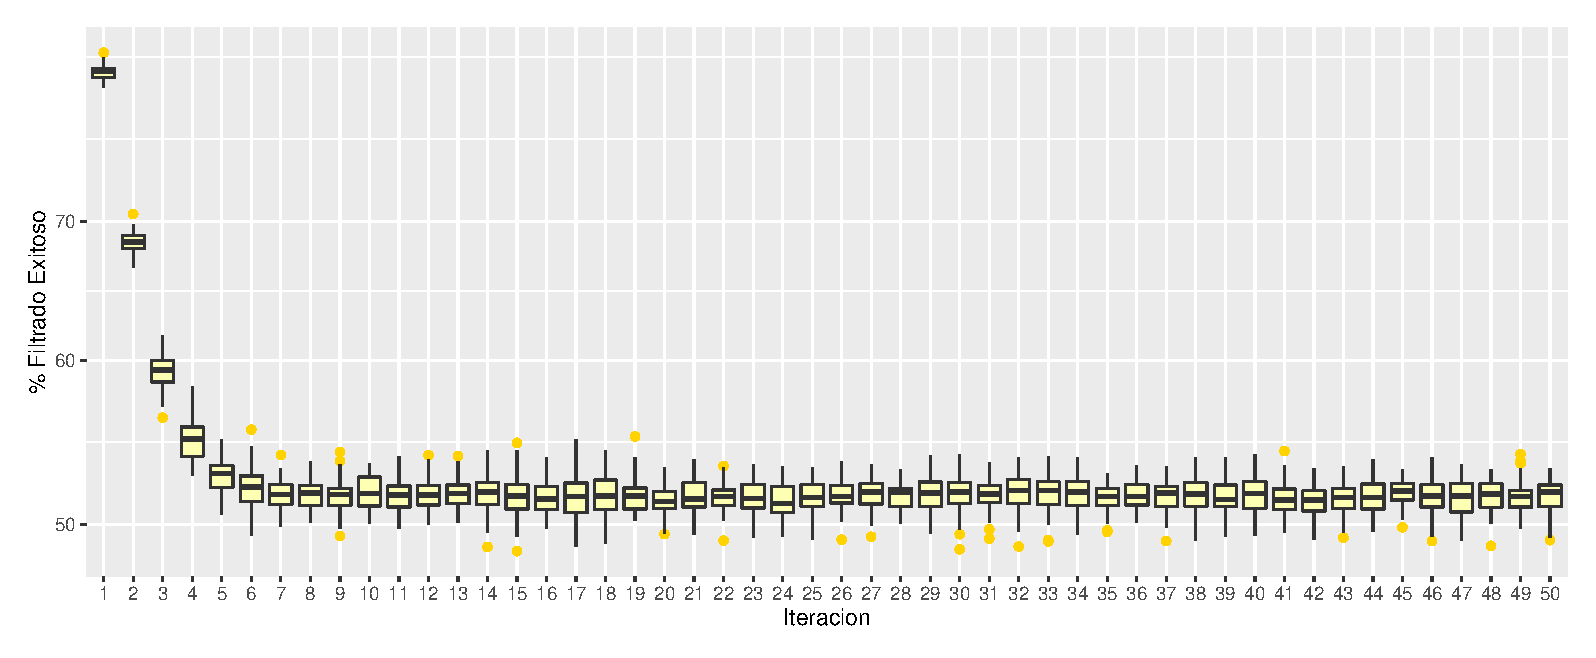
\includegraphics[width=150mm]{k400r2.eps} % archivo
    \caption{k = 400 R2.}
    \label{Figura 6}
\end{figure}
\newpage

%CONCLUSIOOOON
\section{Conclusi\'on Reto}
Comparando las im\'agenes obtenidas despu\'es de modificar el tamaño cr\'itico, podemos observar una notable mejor\'ia en el porcentaje de filtraci\'on.
Por mencionar algunas, si comparamos las gr\'aficas \ref{Figura 1} y \ref{Figura 4}, se observa que en la primer iteraci\'on se alcanzan valores alrededor de 30\% y 65\% respectivamente\cite{symbolporcent}. 
De igual forma se observa con mayor claridad que para los tres grupos de \texttt{k} el momento en que maximiza el porcentaje de filtraci\'on resulta en la primer iteraci\'on.

% BIBLIOGRAFIAAAAAAS
\bibliography{referencias}
\bibliographystyle{plainnat}
\end{document}

